\documentclass[french]{beamer}
\usepackage[round]{natbib}

\usepackage{pgfpages}
%\setbeameroption{show notes}
%\setbeameroption{show notes on second screen=right}
\mode<presentation> {
  \usetheme{Madrid}
  % ou autre ...

  \setbeamercovered{transparent}
  % ou autre chose (il est également possible de supprimer cette ligne)
}
\newtheorem{proposition}[theorem]{Proposition}
\newtheorem{corollaire}[theorem]{Corollaire}

\usepackage[utf8]{inputenc}
\usepackage[T1]{fontenc}
\usepackage{babel}
\usepackage{times}
\usepackage[T1]{fontenc}
\usepackage{tikz}
\usepackage{amsfonts}
%\pgfdeclareimage[height=0.5cm]{le-logo}{logo-irisa}
%\logo{\pgfuseimage{le-logo}}
\setbeamertemplate{footline}[frame number]



%%%%%%%%%%%%%%%%%%%%%%%%%%%
\title{Universalité pour les sous-suites croissantes}

\subtitle {Forum Jeunes Mathématiciennes et Mathématiciens}
\author 
{ \large{Mohamed Slim Kammoun}
\\ Université de Lille \\ \ \\ \large{Avec Mylène Maida  et Adrien Hardy}}
\date { 29 November 2018}
\titlegraphic{

\includegraphics[height=0.9cm]{l1}
   
\includegraphics[height=0.9cm]{0}
   
\includegraphics[height=0.9cm]{l6}
   
}

\begin{document}

\begin{frame}
  \titlepage  
\end{frame}



\section*{Introduction}
\begin{frame}{Introduction}
  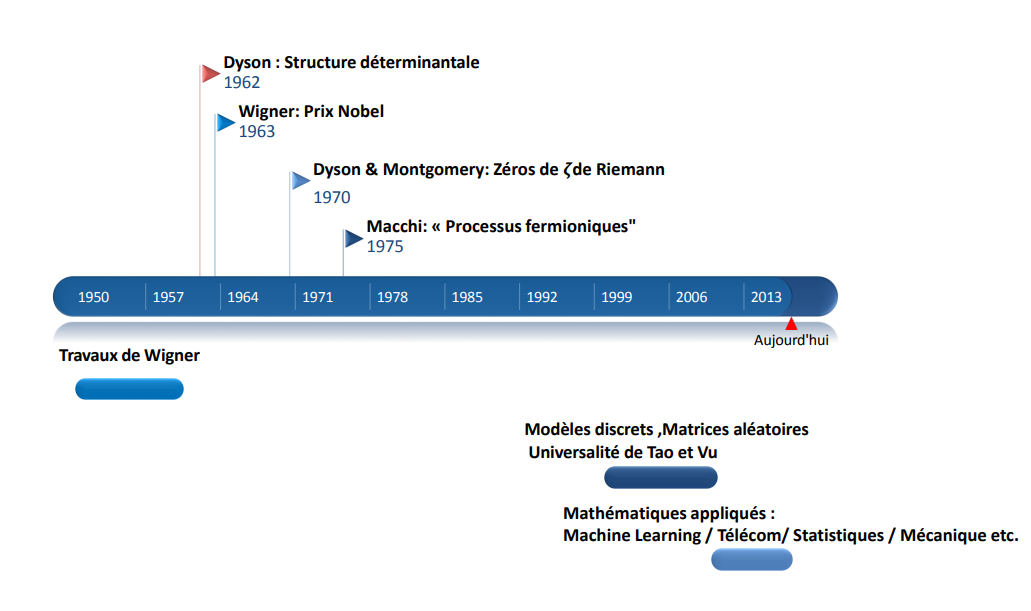
\includegraphics[scale=0.4]{Capture}
\end{frame}
\begin{frame}{Plan}
     \tableofcontents[
    hideothersubsections, 
    sectionstyle=show,
]
\end{frame}



\section{??? }
\begin{frame}{Plan}
\tableofcontents[currentsection,currentsubsection,
    hideothersubsections, 
    sectionstyle=show/shaded,
]
\end{frame}


\subsection{Plus longue sous-suite croissante}
\begin{frame}{Permutations aléatoires}
$\mathfrak{S_n}$ : Le groupe symétrique d'ordre $n$ (l'ensemble des permutations de $\{1,2,\dots,n\}$).
\\ 

\end{frame}
\begin{frame}{Processus ponctuels} 
\begin{definition}[Processus Ponctuel]
Processus ponctuel : Configuration aléatoire
\end{definition}
Exemples :
\begin{itemize}
\item Processus ponctuels de Poisson 
\item Processus ponctuels déterminantaux 
\end{itemize}
\end{frame}
\begin{frame}{Processus ponctuels déterminantaux}

\begin{itemize}

\item $\Xi$: Processus ponctuel
 \item $\mu$ : Une mesure sur $\mathbb{X}$
\end{itemize}

\begin{definition}[DPP]
$\Xi$ est déterminantale si $\exists K$ vérifiant  $\forall k\geq 1,\  \forall f $ continue à support compact . 
  \begin{align*}
  \mathbb{E}(\sum_{{}_{\forall i\neq j, x_i \neq x_j }^{(x_1,...x_k)\in \gamma}} f(x_1,\dots,x_k))=\int_{\mathbb{X}^k}f(x_1,\dots,x_k)\mathrm{det}([K(x_i,x_j)]_{ i,j})d\mu^{\otimes k}
  \end{align*}

\end{definition}
Cas Poisson : \ 
$K(x,y)=\begin{cases}
\lambda(x) & \text{ si } x=y  \\ 
0 & \text{ si } x\neq y 
\end{cases}
$      \end{frame}
\subsection{Diagrammes  et tableaux  de Young}
\begin{frame}{Diagrammes de Young}
\begin{definition}[Diagramme de Young]
$\lambda=(\lambda_i)_{i\geq 1} \in \mathbb{N}^{\mathbb{N}^*}$ diagramme de Young si :
\begin{itemize}
\item  $\lambda_{i+1}\leq \lambda_i$
\item $\exists k \in \mathbb{N}, \lambda_k=0$
\end{itemize}
\end{definition}
\begin{figure}[ht]
    \centering
  \includegraphics[scale=0.17]{1}
\caption {Exemple de diagramme de Young $\lambda=(5,4,1.\underline{0})$}
\end{figure}
\begin{align*}\mathbb{Y}&:\text{l'ensemble des diagrammes de Young}
\end{align*}

\end{frame}

\begin{frame}{Tableaux de Young}

\begin{definition}[Tableaux de Young standards]
Tableau de Young standard: Remplissage d'un diagramme de Young
\begin{itemize}
\item les entrées $\{1,2,3..,\sum_{i\geq 1} \lambda_i \}$ (chacune une seule fois). 
\item croissant sur les lignes et les colonnes.
\end{itemize}
\end{definition}
\begin{align*}
dim(\lambda)&:=  \# \text{Tableau de Young standards}
\\|\lambda|&:=\sum_{i\geq 1} \lambda_i \\  \ell(\lambda)&:=\max_i{\lambda_i>0}
\end{align*}

\end{frame}
\begin{frame}

\section{Processus de Schur}
\tableofcontents[currentsection,currentsubsection, 
    hideothersubsections, 
    sectionstyle=show/shaded,
]
\end{frame}
\subsection{Cas Plancherel}
\begin{frame}{Mesure de Plancherel poissonnisée }
\begin{definition}
soit $\theta>0$
\begin{align*}
\forall \lambda \in \mathbb{Y},  \mathbb{S}_\theta(\lambda):=e^{-\theta^2}\frac{dim^2(\lambda)\theta^{2|\lambda|}}{|\lambda|!^2}
\end{align*}
\end{definition}
\end{frame}
\begin{frame}{Processus ponctuel de Plancherel}

\begin{definition}
soit $\theta>0$
\begin{align*}
\forall \lambda \in \mathbb{Y},  \mathbb{P}_\theta(X(\lambda)):= \mathbb{S}_\theta(\lambda)
\end{align*}
avec $X(\lambda)=\{\lambda_i-i+\frac{1}{2}\}_{i\geq 1}$

\end{definition}
\begin{figure}[ht]
    \centering
  \includegraphics[scale=0.40]{2}
\caption {Exemple de configuration de points  $X((4,2,\underline{0}))$}
\end{figure}
\end{frame}
\begin{frame}{Processus ponctuel de Plancherel : caractère déterminantal}
\begin{theorem}[\cite*{koo00} ; \citep{ok1}]
Le processus ponctuel de Plancherel est déterminantal de noyau $K_\theta$  pour la mesure de contage sur $\mathbb{Z}+\frac{1}{2}$ avec :
\begin{align*}
K_\theta(i,j)=\frac{-1}{4\pi^2} \oint\oint\frac{\exp(\theta(v-w-v^{-1}+w^{-1}))}{(v-w)v^{i+\frac 1 2} w^{-j+\frac 1 2}}\mathrm{d}v 
\end{align*}
\begin{align*}
|w|<|v| \text{ (englobent 0)} 
\end{align*}
\end{theorem}
  \end{frame}

\begin{frame}{Noyau limite "Bulk"}
\begin{theorem}[\cite*{koo00}]
$\forall |u| <2  \ \forall (x,y) \in (\mathbb{Z}+\frac{1}{2})^2$ 
\begin{align*}
\lim_{\theta \to \infty} K_\theta(\lfloor u\theta \rfloor +x, \lfloor u\theta \rfloor +y )&=
\left\{\begin{matrix}
\frac{\phi }{\pi}\  &\text{si }  x=y
\\ 
\frac{\sin(\phi(x-y))}{\pi(x-y)} &\text{sinon} 
\end{matrix}\right.
\\ &:=\tilde{K}_{sin,u}(x,y)
\end{align*}
avec
\begin{align*}
 2cos(\phi)=u
\end{align*}
\end{theorem}
\end{frame}
\subsection{Spécialisations de Schur}
\begin{frame}{Polynômes de Schur}
\begin{definition}[Polynômes de Schur]
$\lambda \in \mathbb{Y}$; $(x_1,\dots,x_N)\in \mathbb{C}^N$
\begin{align*}
s_\lambda(x_1,\dots,x_N):=
\begin{cases}
0 & \text{si } N<\ell(\lambda)
\\ \frac{\mathrm{det}[x_{i}^{\lambda_j+N-j}]_{1\leq i,j\leq N}}{\mathrm{det}[x_{i}^{N-j}]_{1\leq i,j\leq N}} & \text{sinon}
\end{cases}
\end{align*}
\end{definition}
\begin{proposition}
\begin{align*}
\forall \lambda \in \mathbb{Y}; s_\lambda\in \Lambda
\end{align*}
avec $\Lambda $: L'ensemble des polynômes symétriques 
\end{proposition}
\end{frame}

\begin{frame}{Spécialisations de Schur positives}
\begin{definition}[Spécialisation]
Spécialisation : homomorphisme d'algèbre $\Lambda \to \mathbb{C}$  \end{definition}
\begin{definition}[Spécialisation de Schur positive]
Soit $\rho$ une spécialisation. $\rho$ est de Schur positive si : 
$$ \forall \lambda \in \mathbb{Y},\rho(s_\lambda)\geq 0 $$
\end{definition}
\end{frame}
\begin{frame}{Caractérisation des spécialisations de Schur positives}
\begin{proposition}[\cite{OK}]
$\rho$ est de Schur positive ssi $\exists \  \alpha,\beta \in \mathbb{R}_+^{\mathbb{N}^*}$ décroissantes intégrables $\gamma>0$ :
\begin{align*}
\rho(p_1)&=\gamma  + \sum_{i\geq 1} \alpha_i+\beta_i \\
\forall k\geq 2 ,\  \rho(p_k)&=\sum_{i\geq 1} \alpha_i^k-(-\beta_i)^{k}
\end{align*}
avec :
$p_k(x_1,\dots,x_n)=\sum_{i=1}^n x_i^k
$\end{proposition}
On note $\rho=[\alpha,\beta,\gamma]$
\end{frame} 
\begin{frame}{Mesures de Schur}
\begin{definition}[Mesures de Schur , \cite*{ref1}]
Soit $\rho_1$,$\rho_2$  deux spécialisations de Schur positives tels que : 
\begin{align*}
\sum_{\lambda \in \mathbb{Y}} \rho_1(s_\lambda
)\rho_2(s_\lambda) <\infty \end{align*}
On définie:
\begin{align*}
\forall \lambda \in \mathbb{Y}, \mathbb{S}_{\rho_1,\rho_2}({\lambda}):=\frac{ \rho_1(s_\lambda
)\rho_2(s_\lambda)}{\sum_{\mu \in \mathbb{Y}} \rho_1(s_\mu
)\rho_2(s_\mu)}
\end{align*}
\end{definition}
\end{frame}  
\subsection{Processus ponctuels de Schur}
\begin{frame}{Processus ponctuel de Schur}
\begin{definition} [Processus ponctuel de Schur]
Soit $\rho_1$,$\rho_2$  deux spécialisations de Schur positives tels que : 
\begin{align*}
\sum_{\lambda \in \mathbb{Y}} \rho_1(s_\lambda
)\rho_2(s_\lambda) <\infty \end{align*}
On définie:
$\mathbb{P}_{\rho_1,\rho_2}(X(\lambda)):=\mathbb{S}_{\rho_1,\rho_2}(\lambda)$
\end{definition}
Exemple :  $$\mathbb{P}_{[\underline{0},\underline{0},\gamma],[\underline{0},\underline{0},\gamma]}=\mathbb{P}_\gamma$$
\\ On note  $\Xi_{\rho,\rho_2}$ une configuration aléatoire de loi $\mathbb{P}_{\rho_1,\rho_2}$
\end{frame}
\begin{frame}{Caractère déterminantal} 
\begin{theorem}[\cite{ref1}]
Soit $\rho_1=[\alpha_1,\beta_1,\gamma_1]$,$\rho_2=[\alpha_2,\beta_2,\gamma_2]$\\ Si $$\max(||\alpha_1||_\infty,||\alpha_2||_\infty,||\beta_1||_\infty,||\beta_2||_\infty)=r<1$$ alors 
$\Xi_{\rho_1,\rho_2}$ est déterminantal de noyau $K_{\rho_1,\rho_2}$
avec 
\begin{align*} 
K_{\rho_1,\rho_2}(i,j)&=\frac{-1}{4\pi^2} \oint\oint \frac{H(\rho_1,v)H(\rho_2,w^{-1})w^{j- \frac 1 2 }\mathrm{d}v \mathrm{d}w}{H(\rho_1,w)H(\rho_2,v^{-1})(v-w)v^{i+\frac 1 2}}
\\H(\rho,z)&= \exp\left(\sum_{k=1}^\infty p_k(\rho)\frac{z^k}{k}\right) \ ; \  r<|w|<|v|<\frac{1}{r}
\label{H}
\end{align*}
\end{theorem}
\end{frame}
\begin{frame}{Caractère déterminantal}
\begin{corollaire}
Soit $\rho_1=[\alpha_1,\beta_1,\gamma_1]$,  $\rho_2=[\alpha_2,\beta_2,\gamma_2]$\\ Si $\max(||\alpha_1||_\infty,||\beta_1||_\infty)\max(||\alpha_2||_\infty,||\beta_2||_\infty)=R^2<1$ alors 
$\Xi_{\rho_1,\rho_2}$ est déterminantal de noyau $K_{\rho_1,\rho_2}$
avec 
\begin{align*} 
K_{\rho_1,\rho_2}(i,j)&=\frac{-1}{4\pi^2} \oint\oint \frac{H(\rho'_1,v)H(\rho'_2,w^{-1})w^{j- \frac 1 2 }\mathrm{d}v \mathrm{d}w}{H(\rho'_1,w)H(\rho'_2,v^{-1})(v-w)v^{i+\frac 1 2}}
\\ \rho'_1&=[\kappa \alpha_1,\kappa \beta_1,\kappa \gamma_1] , \  \rho'_2=[\frac{1}{\kappa} \alpha_1,\frac{1}{\kappa} \beta_1,\frac{1}{\kappa} \gamma_1] \\
\kappa &=\sqrt \frac{\max(||\alpha_2||_\infty,||\beta_2||_\infty)}{\max(||\alpha_1||_\infty,||\beta_1||_\infty)}\  \ , \ R<w<v<\frac{1}{R}
\end{align*}

\end{corollaire}
\end{frame}
\begin{frame}{Assemptotiques}
\begin{proposition}
$\forall \alpha_1,\alpha_2,\beta_1,\beta_2$ des suites réelles positives décroissantes et sommables $\forall |u| <2  \ \forall (x,y) \in (\mathbb{Z}+\frac{1}{2})^2$ 
\begin{align*}
 K_{[\alpha_1,\beta_1,\theta],[\alpha_2,\beta_2,\theta]}(\lfloor u\theta \rfloor +x, \lfloor u\theta \rfloor +y ) \overset{\theta\to\infty}{\longrightarrow}
\left\{\begin{matrix}
\frac{\phi }{\pi}\  & \text{si } x=y
\\ 
\frac{\sin(\phi(x-y))}{\pi(x-y)} &\text{sinon} 
\end{matrix}\right.
\end{align*}
avec
\begin{align*}
 2cos(\phi)=u
 \end{align*}
\end{proposition}
\end{frame}

\begin{frame}{Assemptotiques}
\begin{proposition}
Soit $f(\theta)=o(\frac{1}{\theta})$, 
\begin{align*}\rho^1(\theta)=[(f(\theta)\mathsf{1}_{i<\frac{\theta}{f(\theta)}}),\underline{0},0]\\ \rho^2(\theta)=[\underline{0},(f(\theta)\mathsf{1}_{i<\frac{\theta}{f(\theta)}}),0]
\end{align*}
$\forall |u| <2  \ \forall (x,y) \in (\mathbb{Z}+\frac{1}{2})^2$
\begin{align*}
 K_{\rho^1,\rho^1}(\lfloor u\theta \rfloor +x, \lfloor u\theta \rfloor +y ) \overset{\theta\to\infty}{\longrightarrow}
\tilde{K}_{sin,u}(x,y)\\ K_{\rho^2,\rho^2}(\lfloor u\theta \rfloor +x, \lfloor u\theta \rfloor +y ) \overset{\theta\to\infty}{\longrightarrow}
\tilde{K}_{sin,u}(x,y)
\end{align*}

\end{proposition}
\end{frame}
\begin{frame}{Statistique linéaire  : nombre de points}
\begin{theorem}
\begin{align*}
\mathbb{E}(\#\Xi_{[\alpha_1,\beta_1,\gamma],[\alpha_2,\beta_2,\gamma]}\cap [0,\infty[)=\frac{2\gamma}{\pi}+O(1)
\end{align*}
\end{theorem}
\end{frame}
\subsection{Rigidité et tolérance}
\begin{frame} {Rigidité} 
\begin{definition}[\cite{gh}]
Soit $\Xi$ un processus ponctuel sur un espace $\mathbb{X}$ , 
$\Xi$ est rigide si 
$\forall C$ pré-compact de $\mathbb{X}, \  \exists f:(\mathbb{X}\setminus C)\to \mathbb{N}  \text{ (déterministe) tels que }$
\begin{align*}
 \#(\Xi\cap C) \overset{p.s}{=} f(\Xi \cap (\mathbb{X\setminus C}))
 \end{align*}
\end{definition}
\begin{theorem}
Le processus ponctuel de noyau sinus discret est rigide (conséquence \cite{Bufetov2016}) 
\end{theorem}

\end{frame}
\begin{frame}{Rigidité}

\begin{theorem}
Le processus ponctuel de Schur est rigide avec 
\begin{align*}
f(\Xi_{ext})=\lim_{n \to \infty} n- \#{\Xi_{ext}}\cap \#[-n,n]
\end{align*}
\end{theorem}
\begin{theorem}
Si $\mathbb{P}(\Xi=X(\mathbb{Y}))=1$ donc $\Xi$ est rigide 
\end{theorem}

Remarque :  la propriété pour C non majoré (mais minoré) 

\end{frame}
\begin{frame}{Tolérance}
\begin{definition}[\cite*{gp}] 

Soit $\Xi$ un processus ponctuel sur $\mathbb{X}$ (muni de $\mu$), $\Xi$ vérifie la propriété "tolérance" si :
$\forall C $ pré-compact, $\forall \Xi_{ext}\in conf(\Xi \setminus C)  $ \\  $\mu.p.s$  $ \forall x_1,x_2....x_n \in C \text{ (deux à deux disjoints)}$ \\ avec $n=f(\Xi_{ext})$ (tolérance)  
\begin{align*}
 \rho_n(x_1,\dots,x_n)>0
\end{align*}
\end{definition}

Dans le cas des processus déterminantaux:
\begin{align*}
\rho_n(x_1,\dots,x_n):=\mathrm{det}([K(x_i,x_j)]_{1\leq  i,j\leq n})
\end{align*}
\end{frame}

\begin{frame}{Tolérance}
\begin{theorem}
On a "Tolérance" des processus de Schur ssi  chaque des deux spécialisations vérifient l'une des propriétés suivantes : 
\begin{itemize}
\item  $\gamma >0 $
\item $\forall i\geq 1 , \alpha_i >0 $ 
\item  $\forall i\geq 1 , \beta_i >0 $
\end{itemize}
\end{theorem}
\end{frame}
\section{Applications}
\subsection{Plus longue sous-suite croissante}
\begin{frame}{Plan}
\tableofcontents[currentsection,currentsubsection, 
    hideothersubsections, 
    sectionstyle=show/shaded,
]
\end{frame}
\begin{frame}{Plus longue sous-suite croissante}
\begin{theorem}[\citeauthor*{BDJ}]
\begin{equation*}
\lim_{\theta \to \infty} \mathbb{S}_\theta\left(\frac{\lambda_1-2\theta}{\theta^\frac 1 3}<s\right)=F_2(s)
\end{equation*}
$F_2(s)$: distribution de Tracy-Widom
\end{theorem}
\begin{corollaire}[\citeauthor*{BDJ}]
\begin{equation*}
\lim_{\theta \to \infty} \mathbb{P}\left(\frac{\mathcal{L}_n-2\sqrt{n}}{n^\frac 1 6}<s\right)=F_2(s)
\end{equation*}
$\mathcal{L}_n$ : plus longue sous-suite croissante d'une permutation aléatoire 
\end{corollaire}
\end{frame}
\subsection{Temps d'embarquement :  modèle d'un seul couloir}
\begin{frame}{Temps d’embarquement : modèle d'un seul couloir }
\begin{block}{Hypothèses}
\begin{itemize}
\item<1-2> Un seul couloir et  un seul escalier  
\item<1-2> Permutation uniforme des passagers
\item<1-2> Temps d'installation constant 
\item<1-2> Temps d'avance négligeable (par rapport au temps  de l'installation)
\item<2> Chaque passager attend tout autre passager de même rangée ayant monté avant  lui 
\end{itemize}
\end{block}
\begin{align*}
\lim_{n\to \infty}
\mathbb{P}( \onslide<2->{c_{n,k}}t_n <2\sqrt{n}+sn^\frac 1 6) = F_2(s)  
\end{align*}
\end{frame}
\begin{frame}{Simulation}
\begin{figure}[ht]
    \centering
  \includegraphics[scale=0.30]{5}
\caption {Configuration A320 , 180 sièges (Air France)}
\end{figure}
\begin{figure}[ht]
    \centering
  \includegraphics[scale=0.35]{6}
\caption {Simulation pour A320 , 180 sièges (Air France)  }
\end{figure}
\end{frame}

\subsection{Temps d’embarquement : modèle de deux couloirs}
\begin{frame}{Temps d’embarquement : modèle de deux couloirs  }
\begin{block}{Hypothèses}
\begin{itemize}
\item<1-2> Deux couloirs
\item<1-2> Permutation uniforme des passagers 
\item<1-2> Temps d'installation constant négligeable par rapport à l'attente d'installation des autres passagers 
\item<2> Tout passager attend tout autre passager du même rangée ayant monté avant lui
\item<2> Distribution symétrique des sièges pour les deux couloirs 
\end{itemize}
\end{block}
\begin{align*}
\lim_{n\to \infty}
\mathbb{P}( \onslide<2->{C_{n,k}}t_n^{(2)}< \sqrt{2n}+sn^\frac 1 6) = F^{2}_2(2^\frac{1}{6}s)  
\end{align*}

\end{frame}
\begin{frame}{Simulation}
\begin{figure}[ht]
    \centering
  \includegraphics[scale=0.30]{7}
\caption {Configuration A380-800, 449 sièges (Emirates)}
\end{figure}
\begin{figure}[ht]
    \centering
  \includegraphics[scale=0.35]{8}
\caption {Simulation pour A380-800, 449 sièges (Emirates)}
\end{figure}
\end{frame}

\section{Travaux en cours}
\begin{frame}{Plan}
\tableofcontents[currentsection,currentsubsection, 
    hideothersubsections, 
    sectionstyle=show/shaded,
]
\end{frame}
\begin{frame}{Plus longue sous-suite croissante : loi d’Ewens}
\begin{figure}[ht]
    \centering
  \includegraphics[scale=0.55]{9}
\caption {Plus longue sous suite-croissante sous loi d’Ewens $n=1000$, $\theta=0.1$
}
\end{figure}
\end{frame}

\begin{frame}{Plus longue sous-suite croissante : loi d’Ewens}
Apparition de noyau sinus limite (Loi d’Ewens +RSK)
\begin{figure}[ht]
    \centering
  \includegraphics[scale=0.4]{10}
\caption {Simulation de la première fonction de corrélation}
\end{figure}

\end{frame}

\begin{frame}{Processus de Schur}
\begin{itemize}
\item  Théorèmes limites fonctionnels (sinus discret)
\item  Statiques linéaires et contrôle de variance
\item Cas $\max
 (||\alpha_1||_\infty,||\beta_1||_\infty)$ * $\max
 (||\alpha_2||_\infty,||\beta_2||_\infty) =1 $
\item Mesures de Palm réduites.
\item Processus liés ((Push-)TASEP, Mots aléatoires etc.)
\item Relation avec les motifs de Gelfand-Tsetlin
\end{itemize}
\end{frame}

\begin{frame}{Processus de Macdonald}

\begin{itemize}
\item  Rigidité
\item  Tolérance
\item  Mesures de Palm
\item Caractérisation des spécialisations de Macdonald positives 
\end{itemize}
\end{frame}

\section*{Conclusion}
\begin{frame}{Conclusion}
\begin{itemize}
\item \textcolor{blue}{ Universalité} : apparition du noyau sinus 
\item \textcolor{blue}{Rigidité}
\item \textcolor{blue}{Tolérance}: caractérisation 
\item \textcolor{blue}{Application} : loi de temps d'embarquement 
\item \textcolor{blue}{Généralisations} : Macdonald, loi d'Ewens  etc.
\end{itemize}
\end{frame}

\begin{frame}{Références}
\tiny

\bibliographystyle{abbrvnat}
    \bibliography{test}

\end{frame}
\begin{frame}

  \begin{columns}
    \begin{column}{0.70\textwidth}
      \begin{center}
        \includegraphics[width=\textwidth]{11}          
      \end{center}
    \end{column}
    \begin{column}{0.30\textwidth}
      \begin{center}

        \font\endfont = cmss10 at 5.40mm
\color[rgb]{0.00,0.00,1.00}       \endfont 
        \baselineskip 7.0mm

        Merci de votre attention

      \end{center}    

    \end{column}
  \end{columns}

\end{frame}


\end{document}